\section{Control}
El diagrama de control de un robot industrial representa cómo se procesa la información desde que el usuario define lo que quiere que haga el robot, hasta que este ejecuta el movimiento real. Se puede dividir en tres bloques principales: la planificación de trayectoria, la cinemática inversa y la dinámica del robot.

Primero, el usuario define los valores que quiere que alcance el efector final del robot. Estos valores pueden ser las coordenadas de los puntos que debe seguir, la velocidad máxima, la aceleración máxima y el tipo de trayectoria. Esta información entra al bloque de planificación de trayectoria, donde se generan los valores que describen cómo debe moverse el efector final, como su posición, velocidad y aceleración, tanto lineal como angular.

Luego, esta información pasa a la parte de la cinemática inversa. Ahí se transforma en variables articulares, es decir, se calculan las posiciones, velocidades y aceleraciones que deben tener las articulaciones del robot para que el efector final logre seguir correctamente la trayectoria deseada.



\begin{figure}[h]
	\centering
	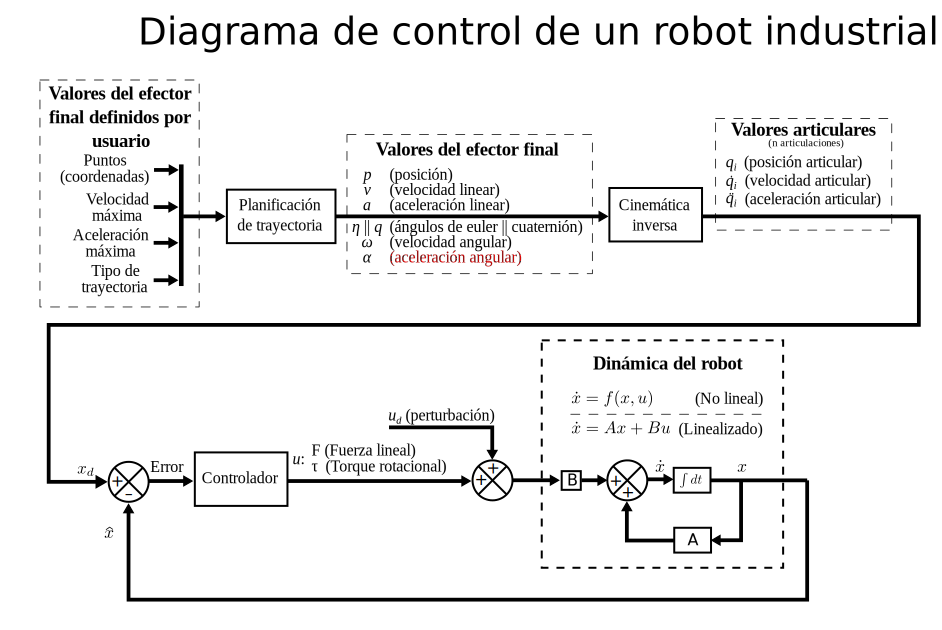
\includegraphics[width=\linewidth]{img/Diagrama_robot_industrial}
	\caption{Diagrama de bloques de un robot industrial}
	\label{fig:diagrama-de-robot-industrial}
\end{figure}

Después, se entra al bloque de dinámica del robot. Aquí se consideran los efectos físicos del movimiento, como la masa del robot, la inercia, las fuerzas y los torques necesarios para lograr el movimiento. También se toman en cuenta posibles perturbaciones externas que podrían afectar el comportamiento del robot, como fricción o impactos. El modelo dinámico puede analizarse en su forma más completa o como una versión simplificada y linealizada para facilitar el diseño del controlador.

El controlador compara el estado actual del robot con el estado que se desea alcanzar. Si hay diferencia, o error, el controlador genera una acción de control, que puede ser una fuerza o un torque, para corregir ese error. Todo este proceso ocurre de forma continua, actualizándose en tiempo real para asegurar que el robot siga la trayectoria correcta, incluso cuando existan perturbaciones o condiciones externas cambiantes.

En resumen, el diagrama muestra cómo se integra la información del usuario con las leyes del movimiento y el control automático para que el robot industrial pueda realizar tareas de manera precisa y eficiente.
\cite{fundamentosRobotica}
\cite{introduccionRobotica}



